\section{Experimental Results}

\mypar{Experimental Setup} Measurements were done on a Lenovo ThinkPad T430s
with 8 Gigabytes of RAM. The operating system being used is the 64-bit variant
of Kubuntu 14.04. The compiler being used is the GNU C Compiler, version 4.8.2.
The following flags were used for compilation:

\begin{verbatim}
-O3 -m64 -march=corei7-avx -Wall\
  -mavx -fno-tree-vectorize
\end{verbatim}

Details about the processor can be found in the table below:

\begin{table}[H]
\begin{center}
\begin{tabular}{>{\bfseries}ll}
Manufacturer         & Intel Corp.\\
CPU Name             & Core i7-3520M\\
L1-Cache             & 32 KB\\
L2-Cache             & 256 KB\\
L3-Cache             & 4 MB\\
No. of cores         & 2\\
CPU-core frequency   & 2901 MHz\\
Scalar FP-Add Cycles/issue  & 1\\
Vect. FP-Add Cycles/issue (SSE) & 2\\
Vect. FP-Add Cycles/issue (AVX) & 4\\
Peak Performance     & 2.9 GFLops/s $\hat{=}$ 1 add/cycle
\end{tabular}
\end{center}
\caption{Processor details.}
\label{tblProc}
\end{table}

In the above table, we only consider the peak performance with respect to
floating point additions since our algorithm does not perform any other floating
point operations.

To asses the performance, libperfmon
4\footnote{\url{http://perfmon2.sourceforge.net/}} was used to measure the
number of cycles. The results were obtained by averaging over 10 consecutive
executions for a given problem size.

To obtain the measurement data for the roofline-plots, perfplot was used,
together with libpcm 2.6.

There is a crucial difference between the performance plots and the roofline
plots: For the latter all floating point operations were counted, including
comparisons, whereas for the former, the number of additions from the cost
analysis was used as a basis.

\begin{figure}[htb]\centering
  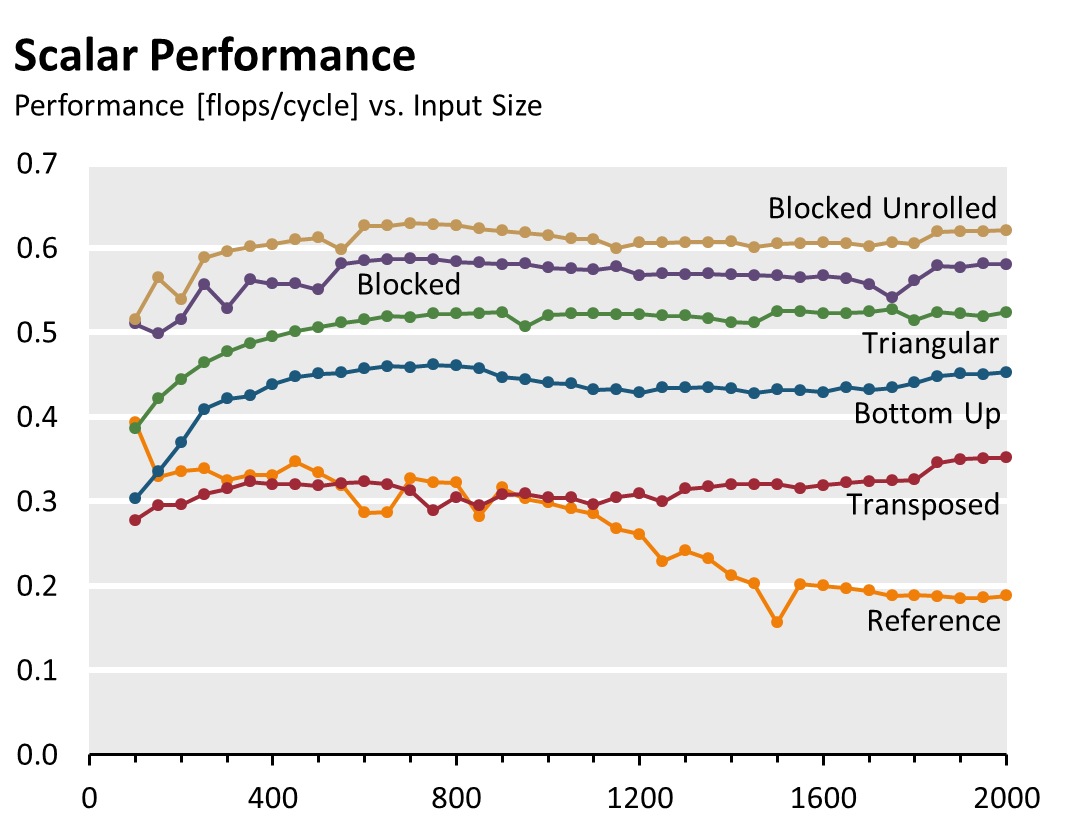
\includegraphics[width=\linewidth]{plot_data/scalar_performance.png}
  \caption{Performance of the scalar implementations.}
  \label{fig:perf-scalar}
\end{figure}

\autoref{fig:perf-scalar} compares the performance of the different scalar
implementations. For the vectorized implementations, we consider the two
\emph{branches}: the implementations based on Triangular- and those based the
Blocking-approach.

\begin{figure}[htb]\centering
  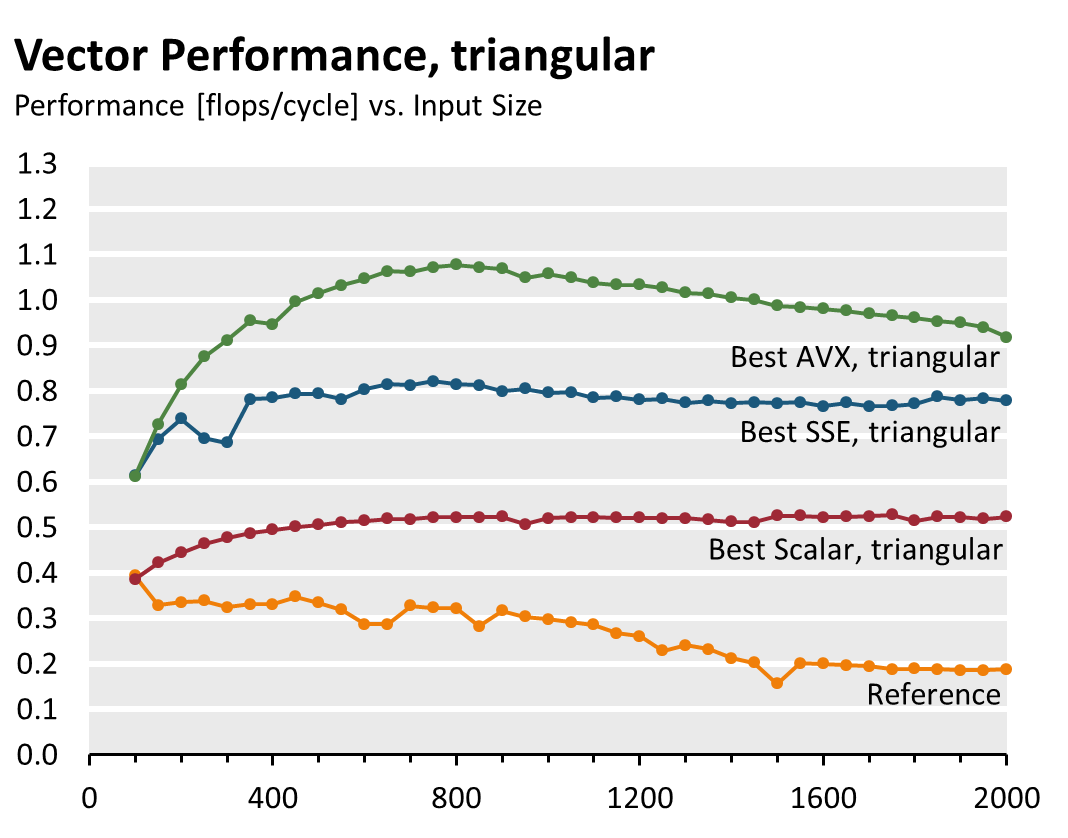
\includegraphics[width=\linewidth]{plot_data/triangular_vector_performance.png}
  \caption{Vectorization based on Triangular.}
  \label{fig:perf-triangular}
\end{figure}

The Triangular version 

\begin{figure}[htb]\centering
  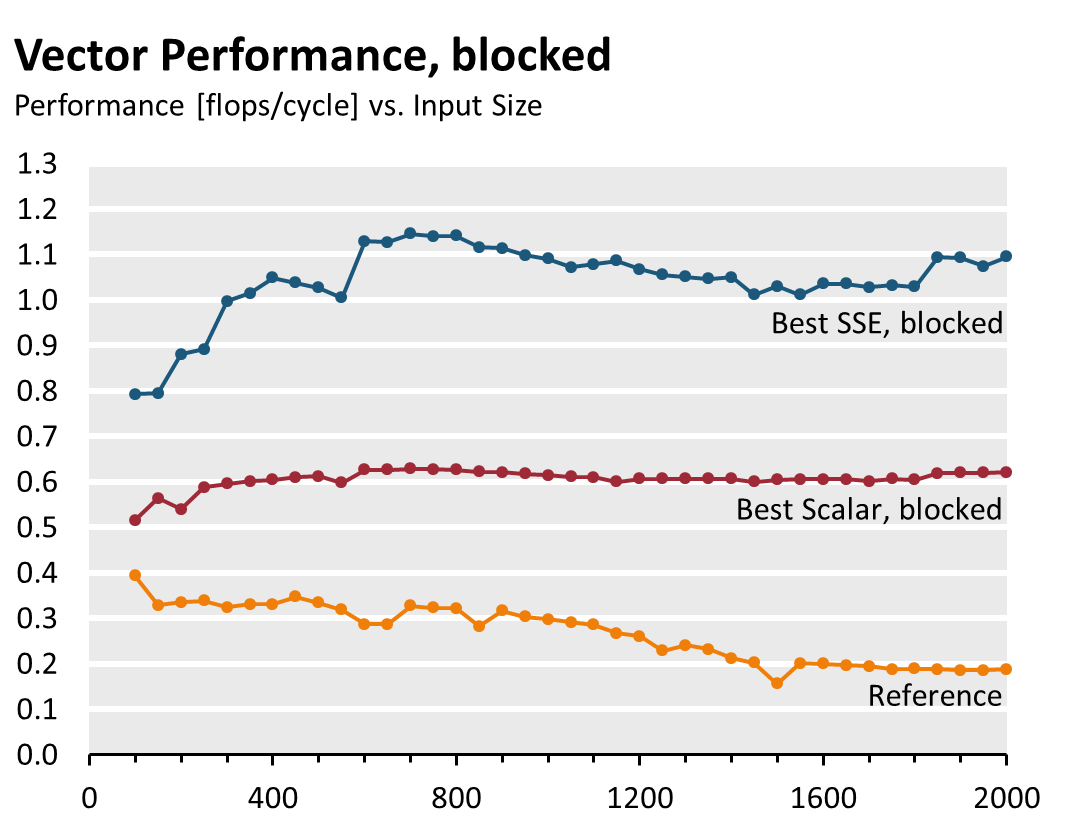
\includegraphics[width=\linewidth]{plot_data/blocked_vector_performance.png}
  \caption{One code to rule 'em all.}
  \label{fig:perf-blocked}
\end{figure}
\begin{figure}[htb]\centering
  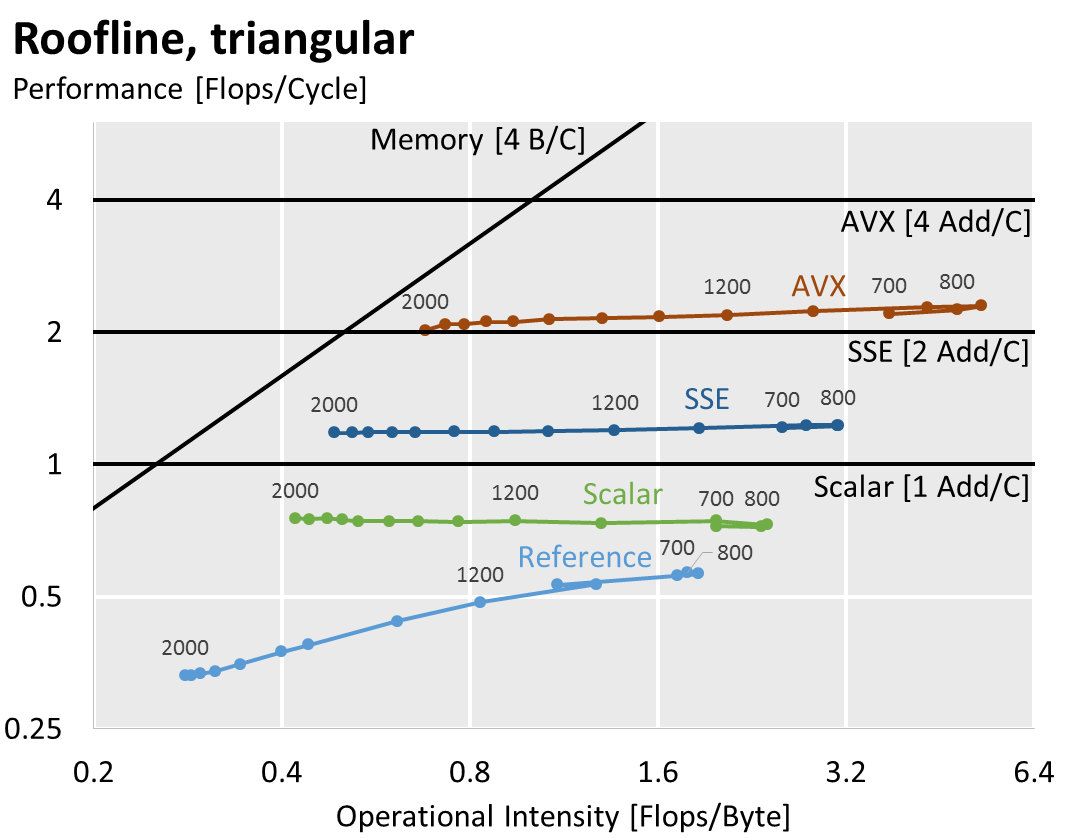
\includegraphics[width=\linewidth]{roofline-data/roofline_triangular.png}
  \caption{One code to rule 'em all.}
  \label{fig:roofline-triangular}
\end{figure}
\begin{figure}[htb]\centering
  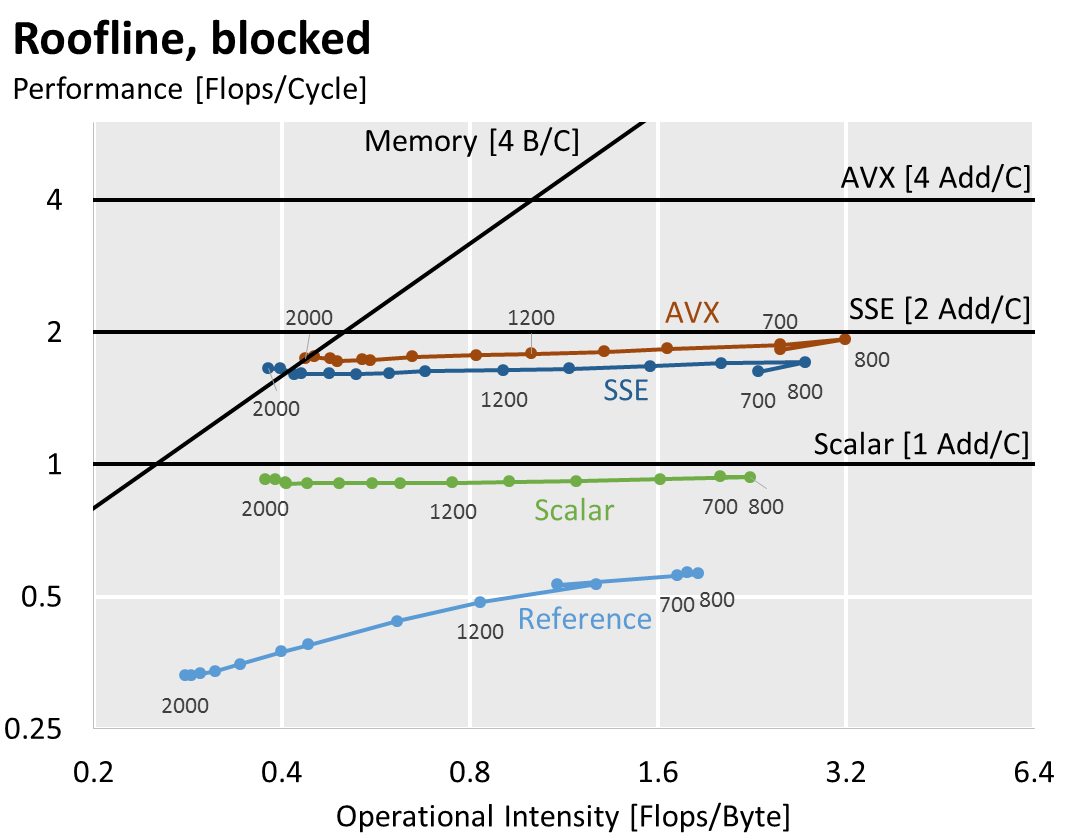
\includegraphics[width=\linewidth]{roofline-data/roofline_blocked.png}
  \caption{One code to rule 'em all.}
  \label{fig:roofline-blocked}
\end{figure}
